\documentclass[11pt, a4paper]{article}
\usepackage{graphicx} % Required for inserting images
\graphicspath{{images/}} % Configuring the graphicx package
\usepackage[a4paper, total={6.5in, 10in}]{geometry}

\title{Anforderungsliste PREN 1}
\author{Team 10}
\date{September 2024}

\begin{document}

\maketitle

\section{Anforderungsliste}
\textbf{Legende} \\ F = Festanforderung \\ M = Mindestanforderung \\ W = Wunschanforderung


\subsection{Allgemeine Anforderungen}
    \begin{tabular}{|l|l|l|l|}
    \hline
    & \textbf{F} & & \textbf{Daten} \\
    \textbf{Nr.} & \textbf{M} & \textbf{Bezeichnung} & \textbf{Werte} \\
    & \textbf{W} & & \textbf{Erläuterungen} \\
    \hline
    1.1 & W & Wettbewerb & Team 10 wird im Wettbewerb einen Podestplatz erreichen. \\
    \hline
    1.2 & F & Wettbewerbsort & Vorraussichtlich wird der Wettbewerb im Foyer der \\
    & & & Mensa durchgeführt. \\
    \hline
    1.3 & F & Projektbewertung & Das Projekt wird anhand der folgenden Punkten \\
    & & & bewertet: \\
    & & & 1. Wettbewerbserfolg \\
    & & & 2. Zuverlässigkeit der Lösung \\
    & & & 3. Nachhaltigkeit und Life-Cycle-Design \\
    \hline
    1.4 & F & Eigenkonstruktion & Einzelne Systemkomponenten wie z.B. Räder, Servos, \\
    & & & Motoren, Mikrocontroller, Kamera, etc. dürfen zugekauft \\
    & & & und eingesetzt werden. Das zu realisierende Fahrzeug \\
    & & & als Grosses und Ganzes muss jedoch zwingend eine \\
    & & & Eigenkonstruktion sein. \\
    \hline
    1.5 & F & Software & Es dürfen Software-Komponenten und Software-Services \\
    & & & von Fremd-Herstellern verwendet werden. \\
    \hline
    1.6 & F & Eingriffe & Ein Eingreifen auf das Fahrzeug ist nach dem Start nicht \\
    & & & mehr erlaubt. \\
    \hline
    1.7 & F & Sicherheit & Das Team ist während sämtlichen Betriebs- und \\
    & & & Test-Phasen verantwortlich für die Sicherheit des \\
    & & & Fahrzeuges und den Schutz der Personen. \\
    \hline
    \end{tabular}
    

\subsection{Gerät}
    \begin{tabular}{|l|l|l|l|}
    \hline
    & \textbf{F} & & \textbf{Daten} \\
    \textbf{Nr.} & \textbf{M} & \textbf{Bezeichnung} & \textbf{Werte} \\
    & \textbf{W} & & \textbf{Erläuterungen} \\
    \hline
    2.1 & F & Autonomität & Das Fahrzeug muss den vorgegebenen Parcours von Start \\
    & & & bis Ziel ohne Zugriff von aussen absolvieren können. \\
    \hline
    2.2 & F & Hardware- & Alle zum Betrieb benötigten Hardware-Komponenten wie \\
    & & Komponenten & z.B. Sensoren, Aktoren, Steuergeräte, Kamera, etc. \\
    & & & müssen sich im oder auf dem Fahrzeug befinden. \\
    \hline
    2.3 & M & Betriebsbereitschaft & Das Fahrzeug muss innerhalb von maximal einer Minute \\
    & & & im Startbereich platziert, aufgebaut und betriebsbereit \\
    & & & sein konnen. \\
    \hline
    2.4 & F & Hindernisbehandlung & Befährt das Fahrzeug eine Strecke mit einem Hindernis, \\
    & & & so muss dieses erkannt und aktiv von der Strecke \\
    & & & aufgenommen werden. Sobald das Fahrzeug die besagte \\
    & & & Stelle passiert hat, muss das Hindernis wieder an die \\
    & & & Ursprungsposition zurückgestellt werden. Die \\
    & & & Toleranzzone beim zurückstellen des Hindernis beträgt \\
    & & & 20 mm (umlaufend). \\
    \hline
    2.5 & F & Zielposition & Die Zielposition (1, 2 oder 3) muss am Fahrzeug mittels \\
    & & & einem Wahlschalter ausgewählt werden können. \\
    \hline
    2.6 & F & Startbefehl & Der Startbefehl wird mittels einem Schalter oder Taster \\
    & & & am Fahrzeug erteilt. (Gleichzeitig wird die Sicht auf \\
    & & & die Strecke freigegeben und die Zeitmessung gestartet) \\
    \hline
    2.7 & F & Leitlinien & Das Fahrzeug muss sich während dem gesamten Parcours \\
    & & & auf den vorgegebenen Leitlinien bewegen. \\
    \hline
    2.8 & F & Not-Aus & Das Fahrzeug muss über einen leicht zugänglichen \\
    & & & Not-Aus-Knopf oder -Schalter verfügen, der alle \\
    & & & mechanisch-dynamische Prozesse sofort unterbricht. \\
    \hline
    2.9 & M & Gewicht & Das Fahrzeug darf das Maximalgewicht von 2kg nicht \\
    & & & überschreiten. \\
    \hline
    2.10 & M & Dimensionen & Das Fahrzeug darf die Dimensionen des Startbereichs \\
    & & & (30 x 30 cm) nicht überschreiten. Zudem ist die Höhe \\
    & & & des Fahrzeugs (oder allfälliger Anbauteile) auf maximal \\
    & & & 80 cm beschränkt. \\
    \hline
    2.11 & F & Zielposition & Das Erreichen der Zielposition muss vom Fahrzeug in \\
    & & & einer passenden Form visuell oder akustisch angezeigt \\
    & & & werden. Zudem muss das Fahrzeug innerhalb eines \\
    & & & Kreises von 30 cm Durchmesser um den Zielpunkt zum \\
    & & & Stehen kommen. \\
    \hline
    \end{tabular}


\subsection{Parcours}
    \begin{tabular}{|l|l|l|l|}
    \hline
    & \textbf{F} & & \textbf{Daten} \\
    \textbf{Nr.} & \textbf{M} & \textbf{Bezeichnung} & \textbf{Werte} \\
    & \textbf{W} & & \textbf{Erläuterungen} \\
    \hline
    3.1 & F & Wege-Netzwerk & Das Wege-Netzwerk und der Startpunkt sind bekannt. \\
    & & & (Figure \ref{fig:wege-netzwerk}) \\
    \hline
    3.2 & F & Zielpunkte & Die möglichen Zielpunkte sind bekannt, doch der \\
    & & & definitive Zielpunkt wird erst unmittelbar vor dem Start \\
    & & & des Parcours bekannt gegeben. (Figure \ref{fig:wege-netzwerk}) \\
    \hline
    3.3 & F & Wegpunkte & Insgesamt gibt es acht Wegpunkte. Die Wegpunkte sind \\
    & & & aufgeklebte Vollkreise (weiss) mit einem Durchmesser \\
    & & & von 7 bis 12 cm. (Figure \ref{fig:wegpunkt}) \\
    \hline
    3.4 & F & Untergrund & Der Untergrund entspricht dem Bodenbelag des Foyers \\
    & & & der Mensa auf dem Campus der Hochschule Luzern für \\
    & & & Technik und Architektur in Horw. (Figure \ref{fig:fliesenboden}) \\
    \hline
    3.5 & F & Leitlinien & Die Wegpunkte sind mit hellen Leitlinien (aufgeklebtes \\
    & & & Klebeband) verbunden. Die Breite der Leitlinien beträgt \\
    & & & ca. 20 mm. \\
    \hline
    3.6 & F & Abmessungen & Der Abstand der Wegpunkte ist variabel zwischen \\
    & & & 0.5 bis 2.0 m. Die Gesamtfläche des Wege-Netzwerkes \\
    & & & beträgt ca. 4.5 x 4.5 m. \\
    \hline
    3.7 & F &  Gesperrte Wegpunkte & Die gesperrten Wegpunkte dürfen nicht befahren werden. \\
    & & & Sie sind bis zum Start unbekannt und mittels einem \\
    & & & Leitkegel gekennzeichnet. \\
    \hline
    3.8 & F & Hindernis auf & Die Strecke darf befahren werden, doch das Hindernis \\
    & & Strecke & muss aktiv von der Strecke aufgenommen und am \\
    & & & gleichen Ort wieder zurückgestellt werden. \\
    \hline
    3.9 & F & Nicht vorhandene & Leitlinien können aus dem Wege-Netzwerk entfernt \\
    & & Teilstrecken & werden. Die entsprechenden Verbindungen können nicht \\
    & & & befahren werden. \\
    \hline
    3.10 & F & Streckenbedingungen & Die Streckenbedingungen (Sperrung, Hindernisse, nicht \\
    & & & vorhandene Teilstrecke) sind bis zum Start unbekannt. \\
    \hline
    3.11 & F & Startbereich & Die Grösse des Startbereichs beträgt 30 x 30 cm. Das \\
    & & & Fahrzeug darf diese Dimensionen nicht überschreiten. \\
    \hline
    3.12 & F & Start & Sobald die Sicht auf die Strecke freigegeben wird, beginnt \\
    & & & ebenfalls die Zeitmessung. \\
    \hline
    \end{tabular}


\subsection{Sensorik}
    \begin{tabular}{|l|l|l|l|}
    \hline
    & \textbf{F} & & \textbf{Daten} \\
    \textbf{Nr.} & \textbf{M} & \textbf{Bezeichnung} & \textbf{Werte} \\
    & \textbf{W} & & \textbf{Erläuterungen} \\
    \hline
    4.1 & F &  Gesperrte Wegpunkte & Die gesperrten Wegpunkte müssen vom Fahrzeug erkannt \\
    & & & werden. \\
    \hline
    4.2 & F & Hindernis auf & Mögliche Hindernisse müssen vom Fahrzeug erkannt \\
    & & Strecke & werden. \\
    \hline
    \end{tabular}


\subsection{Simulation}
    \begin{tabular}{|l|l|l|l|}
    \hline
    & \textbf{F} & & \textbf{Daten} \\
    \textbf{Nr.} & \textbf{M} & \textbf{Bezeichnung} & \textbf{Werte} \\
    & \textbf{W} & & \textbf{Erläuterungen} \\
    \hline
    5.1 & W & Betriebssystem & Die Simulation soll auf Linux und auch Windows ausführbar \\
    & & & sein. \\
    \hline
    5.2 & W & Benutzeroberfläche & Die Benutzeroberfläche soll beliebig editierbar sein. Die \\
    & & & Die gesamte Simulation wird jedoch nur 2-dimensional \\
    & & & realisiert. \\
    \hline
    \end{tabular}


\section{Abbildungen}
Folgend sind sämtliche Abbildungen aufgeführt, auf die in der Anforderungsliste referenziert wurde.

\begin{figure} [ht]
    \centering
    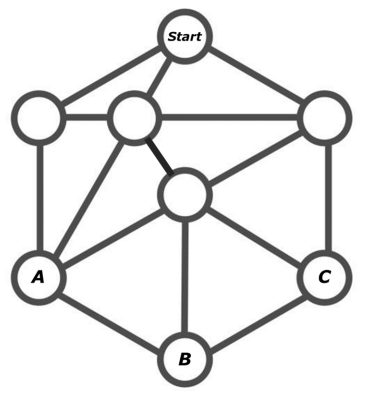
\includegraphics[width=0.4\linewidth]{Images/WegeNetzwerk.png}
    \caption{Vorgegebenes Wege-Netzwerk mit Start- und Zielpositionen A-B-C}
    \label{fig:wege-netzwerk}
\end{figure}

\begin{figure} [ht]
    \centering
    
\includegraphics[width=0.4\linewidth]{Images/Wegpunkt.png}
    \caption{Typischer aufgeklebter Wegpunkt}
    \label{fig:wegpunkt}
\end{figure}

\begin{figure} [ht]
    \centering
    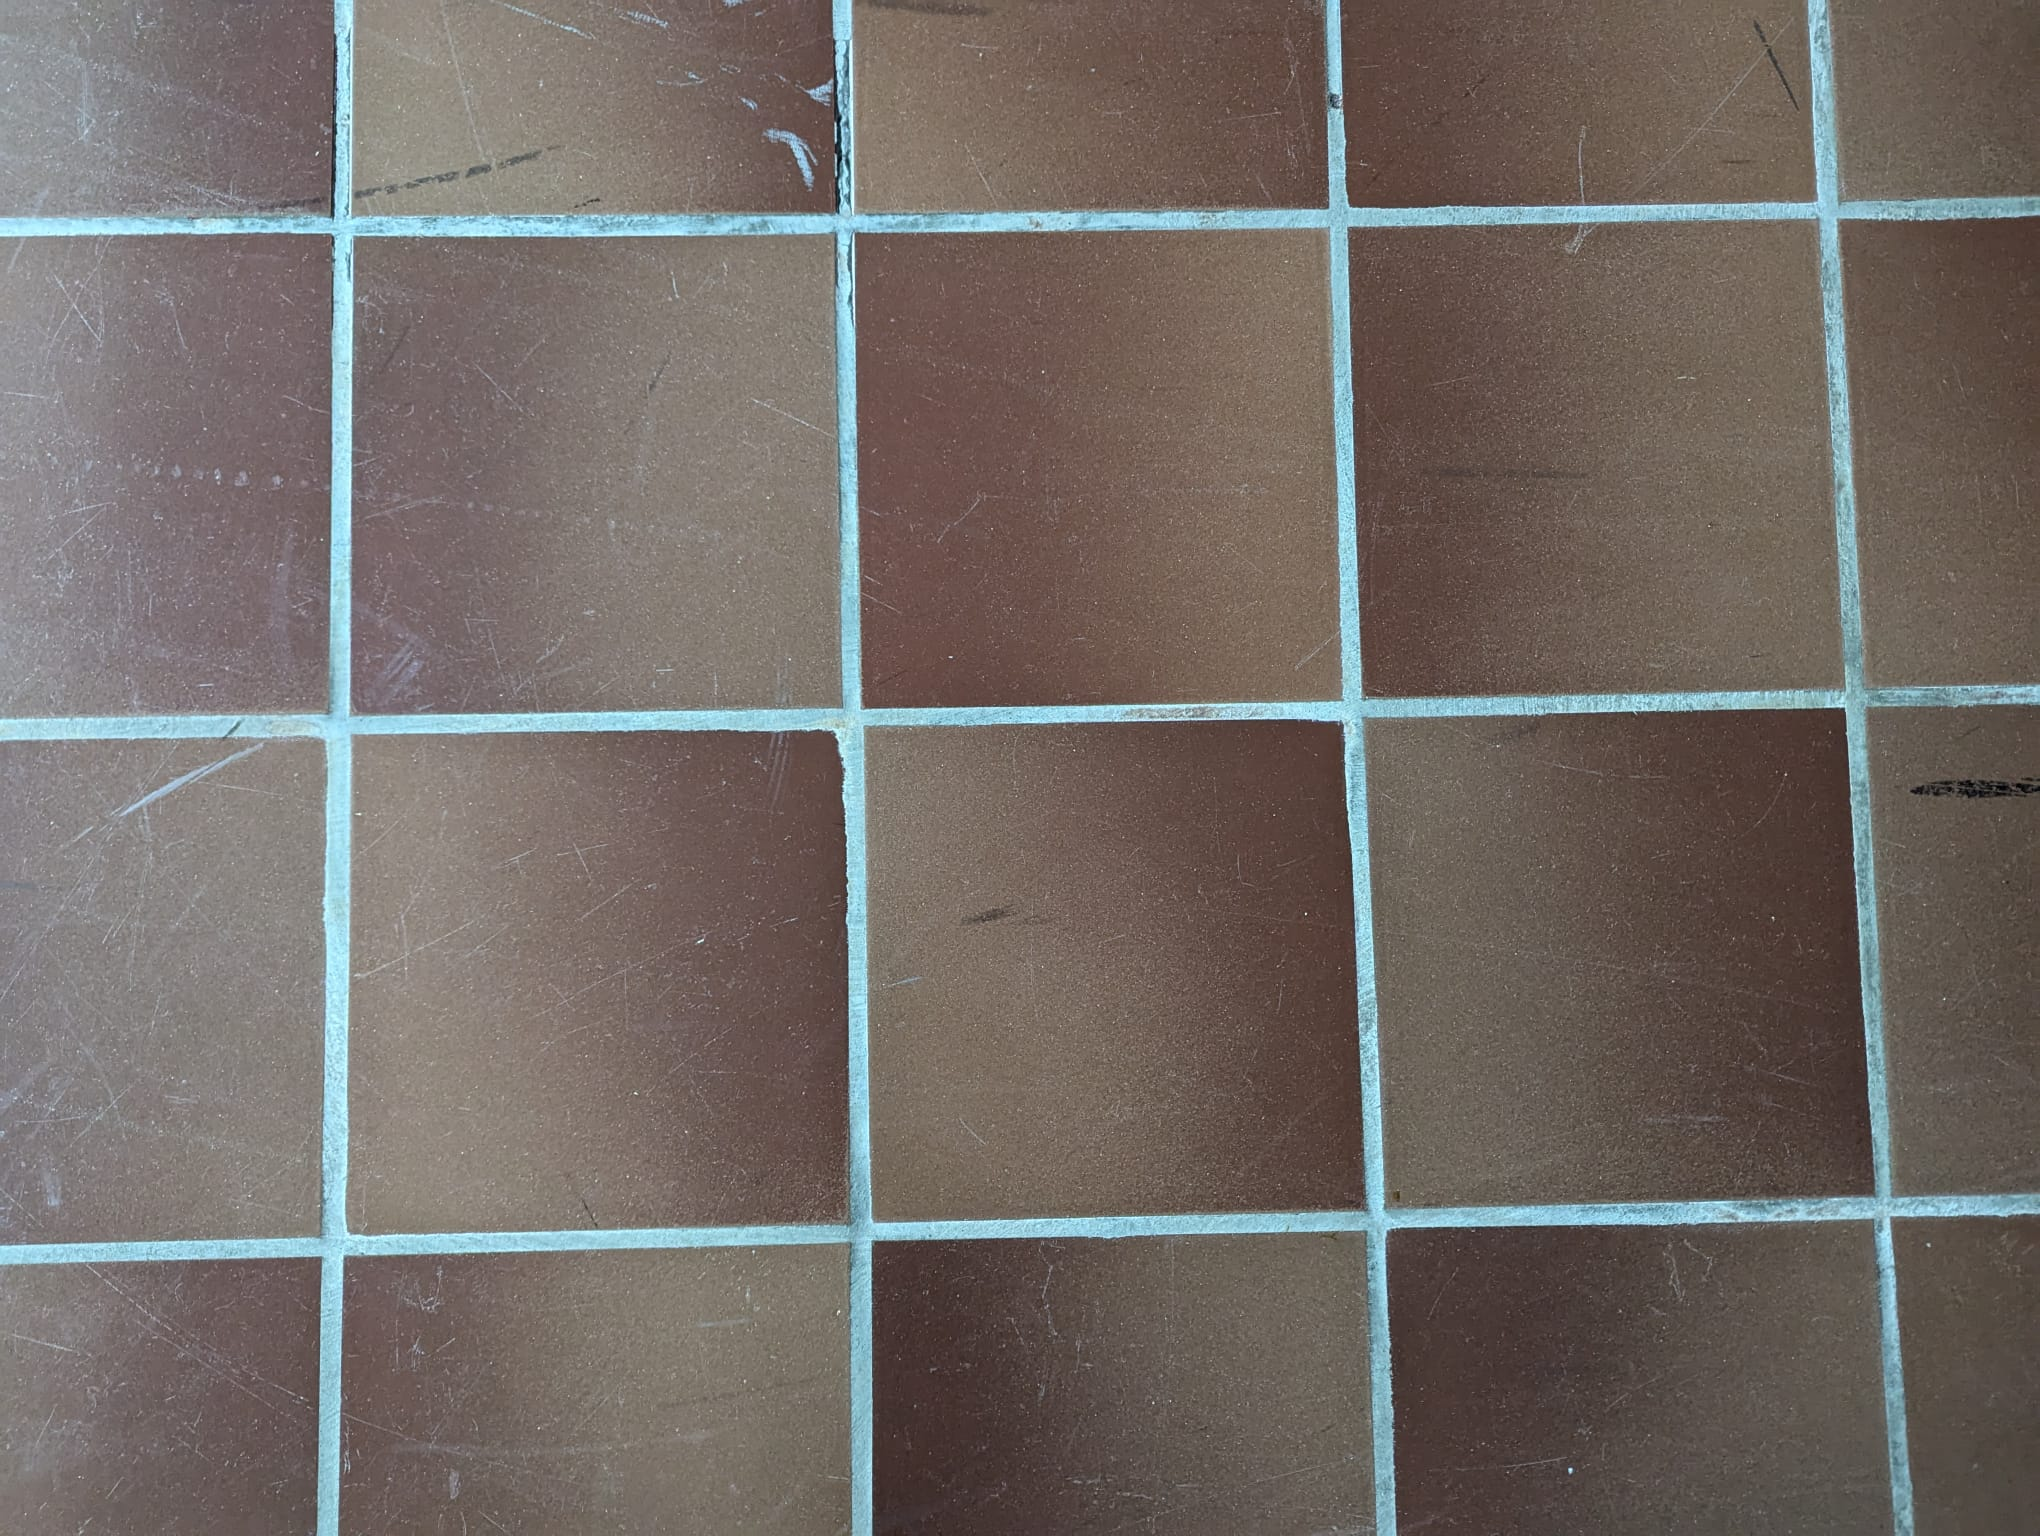
\includegraphics[width=0.4\linewidth]{Images/Fliesenboden.jpg}
    \caption{Fliesenboden im Foyer der Mensa}
    \label{fig:fliesenboden}
\end{figure}

\end{document}
